\section{A MAC Layer in Mote Runner}
\begin{frame}[fragile]
  \frametitle{Design strategy}
  \begin{itemize}
    \item Mac class:
    \begin{itemize}
      \item Coordinator behaviour
      \item Associated node behaviour
    \end{itemize}
    \item Flexible -> functionality on demand
  \end{itemize}

\end{frame}

\begin{frame}[fragile]
  \frametitle{Timing}
  \begin{itemize}
    \item It grants synchronization between mote and coordinator
    \item Realized with a timer and scheduled events
  \end{itemize}
  \begin{figure}
    \centering
    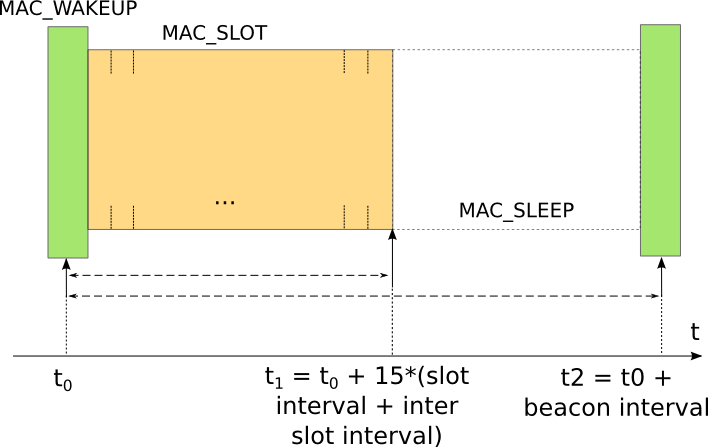
\includegraphics[width=.7\textwidth]{img/MAC_STATES.png}
  \end{figure}

\end{frame}
